\prob
{
    Let $G$ be the directed graph shown in next figure.
            \begin{center}
                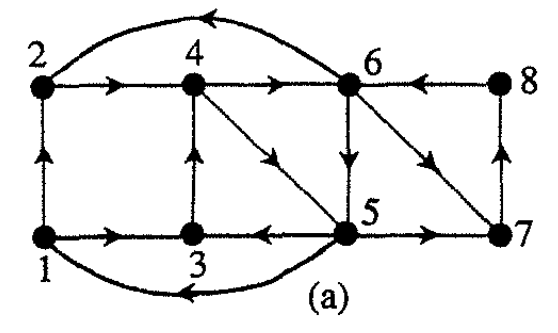
\includegraphics[width=5cm]{Test2/Problem12/DirectedGraphs.png}
            \end{center}\pn
    
    \begin{enumerate}[label=(\roman*)]
        \item   Construct the corresponding bipartite graph $\hat{G}$.
        \item   Let $V = \{1,2,3,4,5,6,7,8\}$, $X=\{5,7\}$, $Y=\{4,2\}$,
                and the paths linking $X$ to $Y$ in $G$ be 5134 and 7862. Construct the
                corresponding matching of $V \setminus X$ to $\hat{V} \setminus \hat{Y}$ in $\hat{G}$.
        \item   Now take the matching $\{2\hat{1}, 3\hat{5}, 4\hat{3}, 5\hat{4}, 6\hat{8}, 8\hat{7}\}$ in $\hat{G}$ and 
                construct the corresponding disjoint paths in $G$ as in the proof of Lemma 2.4.3.
    \end{enumerate}
}
\begin{proof}$\,$\pn

    \begin{enumerate}[label=(\roman*)]
        \item   $\,$\pn  
            \begin{figure}[H]
                \begin{center}
                    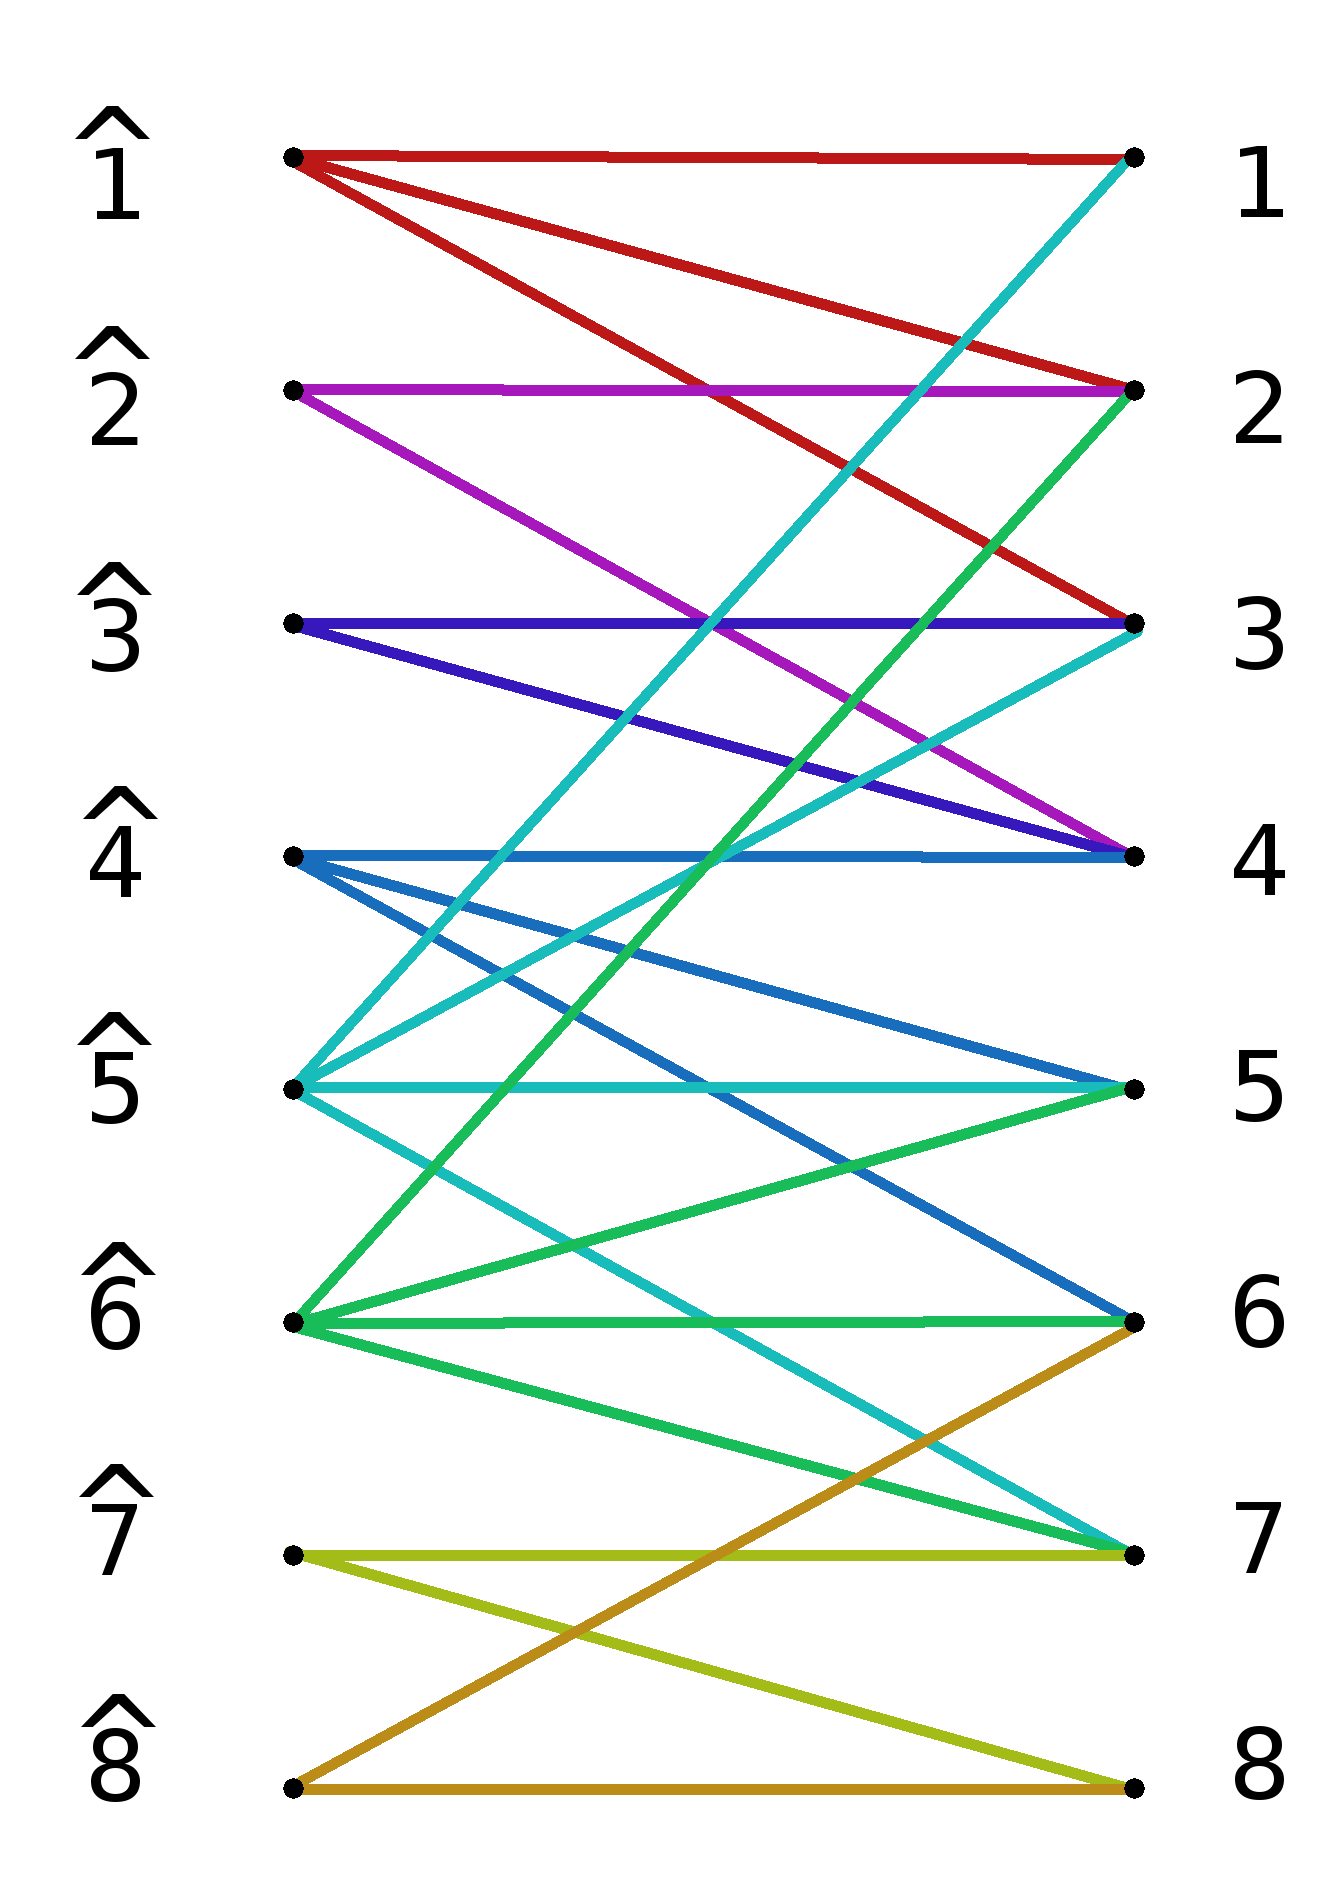
\includegraphics[width=8cm]{Test2/Problem12/BipartiteGraph.png}
                \end{center}                            
                \caption{Bipartite graph}
                \label{t2:p12_BipartiteGraph.png}                        
            \end{figure}\pn 
         \item $\,$\pn  
            \begin{figure}[H]
                \begin{center}
                    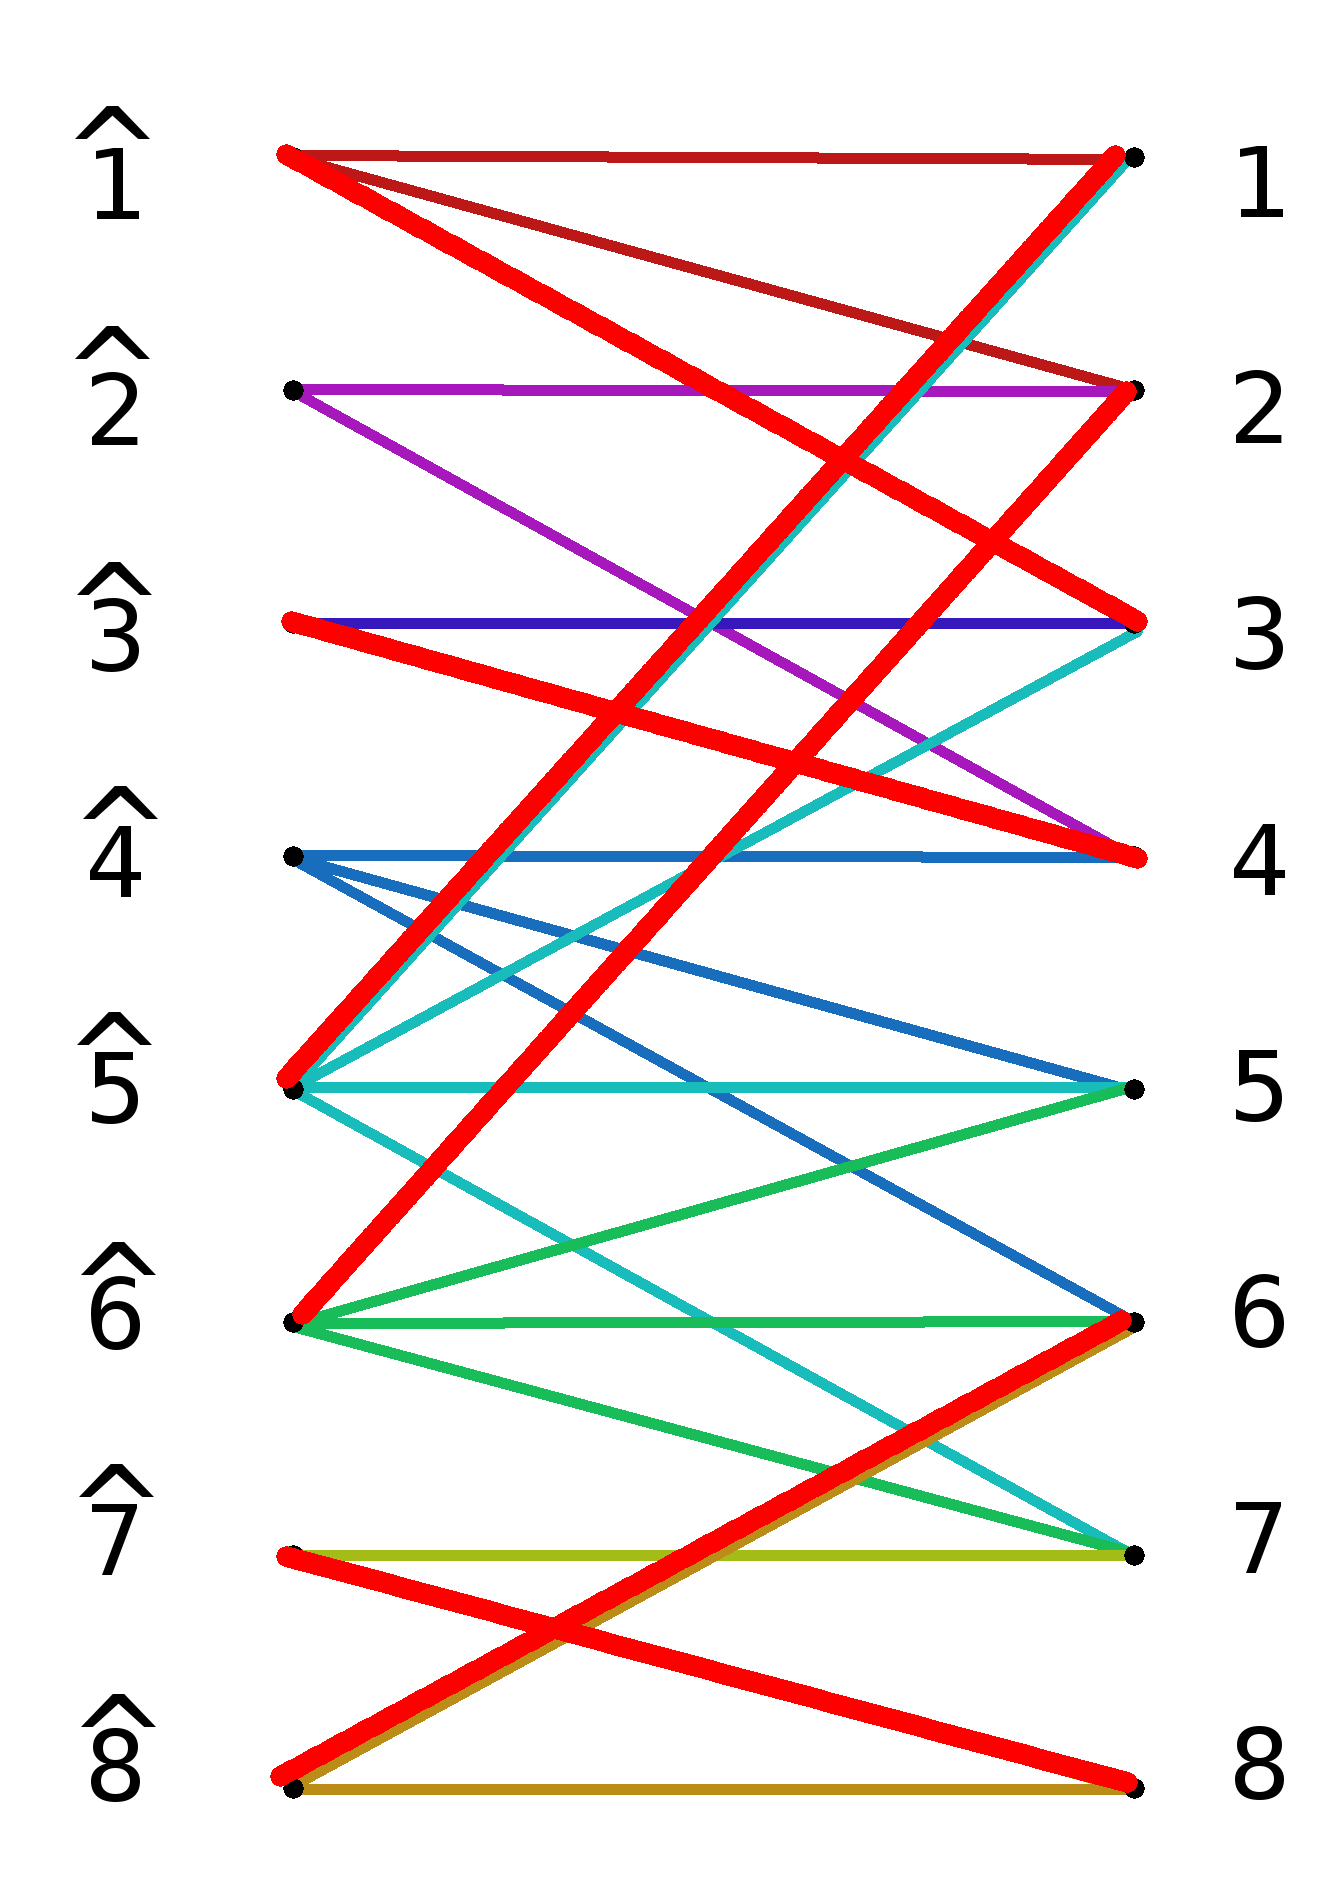
\includegraphics[width=8cm]{Test2/Problem12/BipartiteGraph_Matching.png}
                \end{center}                            
                \caption{Bipartite graph and matching}
                \label{t2:p12_BipartiteGraph_Matching.png}                        
            \end{figure}\pn 
         \item
            The corresponding paths are $(1, 2)$ and $(7, 8, 6)$. It is generated also a cycle
    \end{enumerate}
\end{proof}